\documentclass[11pt]{article}

% Any additional packages needed should be included after jmlr2e.
% Note that jmlr2e.sty includes epsfig, amssymb, natbib and graphicx,
% and defines many common macros, such as 'proof' and 'example'.
%
% It also sets the bibliographystyle to plainnat; for more information on
% natbib citation styles, see the natbib documentation, a copy of which
% is archived at http://www.jmlr.org/format/natbib.pdf

\usepackage{jmlr2e}
\usepackage{hyperref}
\usepackage{bookmark}
\usepackage{setspace} \doublespacing

% todonotes
\usepackage{xargs}                      % Use more than one optional parameter in a new commands
\usepackage[pdftex,dvipsnames]{xcolor}  % Coloured text etc.
\usepackage[colorinlistoftodos,prependcaption,textsize=tiny]{todonotes}
\newcommandx{\unsure}[2][1=]{\todo[linecolor=blue,backgroundcolor=blue!25,bordercolor=blue,#1]{#2}}
\newcommandx{\change}[2][1=]{\todo[linecolor=red,backgroundcolor=red!25,bordercolor=red,#1]{#2}}
\newcommandx{\info}[2][1=]{\todo[linecolor=OliveGreen,backgroundcolor=OliveGreen!25,bordercolor=OliveGreen,#1]{#2}}
\newcommandx{\improvement}[2][1=]{\todo[linecolor=Plum,backgroundcolor=Plum!25,bordercolor=Plum,#1]{#2}}
\newcommandx{\thiswillnotshow}[2][1=]{\todo[disable,#1]{#2}}

% margins for todonotes
\paperwidth=\dimexpr \paperwidth + 6cm\relax
\oddsidemargin=\dimexpr\oddsidemargin + 3cm\relax
\evensidemargin=\dimexpr\evensidemargin + 3cm\relax
\marginparwidth=\dimexpr \marginparwidth + 3cm\relax

% Definitions of handy macros can go here
\usepackage{subfig}
\newcommand{\dataset}{{\cal D}}
\newcommand{\fracpartial}[2]{\frac{\partial #1}{\partial  #2}}

\renewcommand*\contentsname{Table of Contents}

\begin{document}
\title{Syllabify and Conquer: A report on preparing and analysing speech text corpora}
\ShortHeadings{MSc. Project Report Winter 2022, McGill University}{}
\author{Author: Michael Haaf \textit{(michael.haaf@mail.mcgill.ca)} \\ Supervisor: Morgan Sonderegger \textit{(morgan.sonderegger@mcgill.ca)}}

\maketitle
\begin{singlespace}
\tableofcontents
\end{singlespace}
\newpage

\section{Introduction}

\nocite{*}

Natural language is predominantly a spoken phenomena, while the most commons tools for computational natural language processing are predominantly text based. Tools that represent, store, and process audio signals associated with spoken natural language have not always existed and are not trivial to implement relative to comparable text-based processing tools. The reasons for this are straightforward: text-based data is comparably smaller in storage size and less demsnding in memory to process. Moreover, speech-based data have much more complicated metadeta and preprocessing requirements than text-based data, many of these complications being out of the reach of amateur or non-technically proficient researchers. Speech transcription, aligning transcription with speech audio, audio signal processing, and non-uniform metadata/data storage standards are just some of the complications of speech-based natural language processing compared to text-based natural language processing. Given these obstacles, it is not surprising that more tools are researched, written, and developed for text-based corpora than for speech-based corpora in both natural language processing research and industry.

The availability of speech-based corpora and automated tools to make use of them is increasing\footnote{corpora sources , automated alignment , standard variable measurement }, enabling linguists and speech scientists to study spoken language at a much larger scale than previously possible\footnote{large scale studies}. There remains, however, a significant gap between the availability of speech data corpora and their general usability for researchers across disciplines. While libraries like NLTK\cite{noauthor_nltk_nodate} have bridged this gap with large accessible text-based natural language corpora and comprehensive tutorials for their usage, the same does not yet exist for speech data corpora.

This report documents work undertaken over a semester in the MCQLL Lab to perform experiments and develop software to help bridge this gap; particularly to the preparation problems of corpora storage and speech-text alignment. This project focused on the tools PolyglotDB\cite{mcauliffe_polyglot_2017} and Montreal Forced Aligner\cite{mcauliffe_montreal_nodate}, which respectively address the storage and alignment problems described. The steps taken to use these tools for facilitation of a pipeline, from publicly-available corpora acquisition to concrete linguistic analysis, is described technically, demonstrated experimentally, and documented in this report. This report constitutes a technical description of work undertaken with these tools for reproduction, reuse, and as a basis for streamlining the investigation of more advanced linguistics problems that require similar speech data preparation and analysis techniques.

This report additionally describes the software design approaches taken throughout the experimental process to motivate the contribution of the set of tools written by the author and to document their workings for future users, experimenters and developers. These tools are made available in a public repository. Alongside PolyglotDB and Montreal Forced Aligner, they facilitate the generalization of the experimental procedure taken across corpora and languages beyond those covered in the report experiments. This generalization is accomplished by abstracting the differences between corpora (varied in format and language) to a set of configuration files adaptable to the requirements of large sets of known public corpora. Differences in corpora that cannot be abstracted to configuration, especially morphological differences in syllable representation across languages, are implemented using a pattern-based approach, streamlining the introduction of new client logic for new corpora to the adaptation of a testable and flexible template class. This approach aims to contribute a code-base that can dynamically adapt to and reliably implement future client requirements when new corpora necessitate novel business logic in configuration and linguistic structure.

The design approach described arose emergently from the set of challenging problems produced by the varied and rich nature of speech data corpora. These problems surround the automation of various steps in corpora preparation for storage, alignment, and analysis: transcript encoding, audio signal processing, and pronunciation dictionary convention generalization. These problems and their relation to the problems of speech data alignment, storage, and analysis are described in this report, alongside the software contributed to resolve these problems.

\section{Speech Data Preparation Pipeline}

While speech corpora are comprised of substantially the same basic elements across corpora and languages, speech corpora are also complex and heterogeneous in a variety of their features: metadata, directory structure, annotation files, documentation, for just some examples. Dozens of formats have been used to store speech corpora over the past several decades. These variations guarantee that workflow of getting general corpora ready for linguistic analysis is not homogenous -- rather, complications introduced by these variations make manual workflows for general corpus work enormously labour-inducing. Researchers are often required to write scripts in order to make their workflow tenable.

This project indeed required scripting in order to prepare the corpora in question for linguistic analysis. This project used Emergent Design Principles\cite{bain_emergent_2008} to adapt the generalizability of the code written as the complication of the requirements became more clear. More details about the implementation are discussed in \hyperlink{section.4}{Section 5: Software Design}. These practises and principles of software develop aim to allow future investigation into this work to extend the functionality developed during this project easily and reliably.

The result is a speech data preparation pipeline from publically available corpora to aligned speech-text corpora ready for analysis. A small example of the entire approach follows:

\missingfigure{example canto alignments and data shown}

A typical outline of such a problem in general follows. We take corpora from the IARPA (link) dataset as a starting point, though the procedure is general for all speech corpora. IARPA corpora are organized in the following manner:

\begin{singlespace}
\begin{verbatim}
corpus/
|-- scripted/
|   |-- reference_materials/
|   |   |   `-- lexicon.txt
|   |   |   `-- lexicon.sub-train.txt
|   |-- training/
|   |   |-- audio/
|   |   |   `-- recording1.sph
|   |   |   `-- recording2.sph
|   |   |   `-- ...
|   |   |-- transcript_roman/
|   |   |   `-- recording1.txt
|   |   |   `-- recording2.txt
|   |   |   `-- ...
\end{verbatim}
\end{singlespace}


The Montreal Forced Aligner\cite{mcauliffe_montreal_nodate} assumes its own particular format corpus structure:

\begin{singlespace}
\begin{verbatim}
`--pronunciation_dictionary.txt
`--textgrid_corpus/
|   `-- recording1.wav
|   `-- recording1.TextGrid
|   `-- recording2.wav
|   `-- recording2.TextGrid
|   `-- ...
\end{verbatim}
\end{singlespace}

That is, the following steps need to be taken: 

\begin{singlespace}
\begin{itemize}
  \item Convert generic audio files to 16kHz .wav files
  \item .txt transcripts to .TextGrids files, with all text contained in a single time hierarchy (to be updated during alignment)
  \item corpus lexicon to MFA-ready pronunciation dictionary
  \item all of the above for alignment with MFA
\end{itemize}
\end{singlespace}

The following subsections deal with each step of this pipeline in turn, making reference to code used and written throughout, and containing example results within each section.

\subsection{Speech Corpora Acquisition and Organization}

- Download from the internet (discoverability, formats, etc.)
- Occassional need to filter based on what you already have (see the dl.sh script I created that's currently in the google drive)

How about using the test-clean subset of Librispeech? (Defined on the open-slr site). This will mean:
You can make a CSV file with a gender and name corresponidng to each speaker (not much, but it's enough to demonstrate enrichment)
There is a standard amount of speech per speaker (~8 min)
It's a reasonable size for anyone to download (350 M)

And once you have some tutorial output working, we can see if it actually works as a demo (like, is 8 min of speech per person enough to show cool between-speaker differences, or should we do a subset that's ~25 min/person)

I think you jus tneed to download the test-clean subset
then match file names to /media/share/corpora/LibriSpeech
so for example, test-clean/61/70968 has a bunch of flac files starting with 61-70968: 61-70968-0000, etc.
These correspond to files in LibriSpeech on roquefort:
LibriSpeech/61/61-70968-0000.TextGrid and LibriSpeech/61/61-70968-0000.wav
 LibriSpeech/61/61-70968-0001.TextGrid and LibriSpeech/61/61-70968-0001.wav
and so on.  So a little shell scripting is required, but should be fast.  Make sense?
(to spell it out more: what happened at some point was we took the flac file, converted to wav, turned the transcript into a lab file, and aligned the wav and lab using MFA, resulting in a TextGrid .  The lab, wav, and TextGrid files are what's now in the LibriSpeech subdirs. The exact format used for that LibriSpeech dir should let you just point polyglotdb at it as a corpus to import)

\subsection{Transcript to `TextGrid` Conversion}

Praat\cite{noauthor_praat_nodate} TextGrids allows for structuring ‘tiers’ in the TextGrid into the more meaningful hierarchy defined in the database format (e.g. each phone token belongs to a corresponding word).

Generally, transcripts for audio corpora are not made available in TextGrid format. The conversion from general transcript files to TextGrids does not exist, since metadata and formatting can vary from transcript to transcript. This project contributes a general method for specifying the input transcript file properties, such that a variety of audio corporas can have their transcripts converted to the textgrid format. A technical description of this work follows:

The Python library `praatio` \cite{tim_mahrt_praatio_2016} has useful utilities for performing this conversion.

Description/sample usage/results here:

\subsection{Audio Signal Processing}

Aligning audio recordings with text transcriptions is a complicated signal processing task. Uniform standards for time frequency are given by file formant standards (what?? maybe do some reading??).

To align generic audio recordings with generic text transcriptions, there are two prerequisites: a known sampling frequency, and a known file format (What??). In this project, the Montreal Forced Aligner is used, which runs optimally using 16kHz sampling frequency and the .wav audio standard. While many other combinations of frequency and format are possible in principle, some standard must be applied in order for measurement to take place, in turn allowing automated alignment to take place. This section concerns the problem of transforming a large set of audio files to a common sampling frequency and a common file format standard.

For example, the IARPA corpus stores audio files using the `.sph` file format standard, with audio recorded at an 8kHz sample rate. This corpus therefore demonstrates a key example of a corpus needing tranformations in both crucial metrics. Conversion from this format to the standard established above requires scripting: while there exist many tools to convert and resample audio formats, there are none that, crucially, (1) convert arbitrary audio formats to a chosen standard (in this case, .wav); (2) resample .wav from arbitrary sampling frequency to a chosen standard (in this case, 16kHz) without altering the pitch nor speed of the audio file; (3) handle gigabytes of audio files in bulk without running into RAM issues on ordinary machines (16GB RAM).

By point of comparison, the Praat tool can do (1) and (2) but not (3), since Praat scripts, in an effort to produce a non-technical user experience, do not offer memory management or lazy/dynamic loading of audio files at runtime which woudl be required to fulfill requirement (3).



\subsection{Pronunciation Dictionary Production}

As discussed in a previous section, speech-text alignment matches sound to text tokenized upon phonemes. That is, an accurate alignment depends upon reliable decomposition of word pronunciations into constituent phonemes in the text layer. As such, MFA pronunciation dictionaries are two-column files, where the columns represent a one to many mapping from words to pronunciations, and where pronunciations are decomposed into syllables and consituent phonemes by token boundaries.

Speech data corpora under study in this project, such as the IARPA Babel corpus set, typically include a lexicon with a similar mapping as MFA. In the general case, however, the symbols and ordering of phonemes, and of syllabic structure, are nonstandard across corpora. A typical example follows:

\missingfigure{straightforward Canto example}

That is, the word/pronunciation mapping from the IARPA Babel corpus is transformed to an MFA-compatible word/pronunciation mapping for each entry in the IARPA Babel lexicon. This is the general task of the pronunciation dictionary production phase of the speech data preparation pipeline.

Even within a single language and corpora, there can be interesting variation:

\missingfigure{less straightforward canto example}

The variation increases across language and corpora. See the IARPA Lithuanian corporus, for instance:

\missingfigure{example}
\missingfigure{example}

In the more straightforward examples shown above, the problem appears to reduce to simple text manipulations to a standardized character set. The more complicated examples show that the ordering of tokens cannot be strictly assumed: without phonological theory, the ordering of tokens cannot be determined accurately. A brief summary of the necessary syllable structure assumptions follows:\cite{fromkin_introduction_2006}:

Across languages, words are composed of one or more syllables, which are in turn composed of one or more phonemes. Every syllable has a nucleus, which is itself composed of one or more phonemes. Syllable nucleus may be preceeded by one or more phonemes grouped together as an onset, and nucleus may be followed by one or more phonemes grouped together as a coda. Syllables may also have tone/stress indicators, paired with the nucleus vowel.

Further complications arise in determining the boundary between syllabic units. The nucleus may be the first token or the last, and it may itself be composed of more than one token. The bounds of the onset and the coda are dependent on the bounds of the nucleus. A general scheme for syllable unit determination follows:

\begin{itemize}
  \item Coda: all phonemes that occur before the first vowel in the syllable
  \item Nucleus: the first vowel in the syllable, followed by\begin{itemize}\item nothing\item a second vowel \item a sonorant\end{itemize}
  \item Coda: all phonemes that occur after the nucleus
  \item Tone: see below
\end{itemize}

Tone, as indicated above, is more complicated. In this project, tone was often ignored in the early stages in order to produce results faster. However, tone (and related information for nontonal language: stress and pitch) are often included in publically available corpora and are useful for more accurate alignment results to disambiguiate important semantic and pragmatic content.

To demonstrate variation in tone, we can consider IARPA Cantonese and IARPA Lithuanian once again:

\missingfigure{Lithu and Canto tones compared}

While the structure of syllables is finite and tractable in scope, the variation in possible ordering and boundaries of phoneme tokens raises complications in simply reading tokens left to right to assign onset, nucleus, coda, and tone indicators. The software design approached to this problem is described in \hyperlink{section.4}{Section 5: Software Design}.


\subsection{Alignment Production}

Note well: the sample-data/ given in this repository (10 randomly chosen ~10second speech files) is no where near enough data to train a performant model. With this data we are simply verifying that there are no syntax/format issues with your workflow. Once that is verified, you will need to acquire more data to train a performant model. See \href{https://memcauliffe.com/how-much-data-do-you-need-for-a-good-mfa-alignment.html}{this blog post} for rough guidelines as to the magnitude of data required to train a model for alignment/general usage.

The cantonese-scripted Iarpa set has been aligned. Out of ~16000, there were about ~580 "no-speech" files that weren't aligned, as well as about 70 files with speech that weren't aligned. The rest of the set ~15500 seem to have been aligned successfully.

\section{Experiments}

The previous section established a pipeline for turning publically available corpora into aligned speech-text datasets ready for linguistic analysis. In parallel to producing this pipeline and applying it to the IARPA Babel Cantonese and Lithuanian corpora, this project also sought to reproduce basic linguistic analysis on aligned corpora to experiment with and extend the usability of the PolyglotDB platform.

This section outlines the process for taking aligned speech-text datasets. These datasets could be the aligned datasets produced in the pipeline (IARPA Cantonese and Lithuanian). In this case, the Librispeech test-clean dataset, which had already been aligned prior to the experiment phase of this project, was used for these experiments. The process for acquiring the Librispeech test-clean aligned corpora is described in \hyperlink{section.21}{Section 2.1: Speech Corpora Acquisition}. The choice of this corpos both permitted parallel work on the data preparation pipeline, and facilitated easier comprehension of the linguistic analysis for general audiences, including the author himself.

This section begins with reproductions of existing PolyglotDB tutorials to demonstrate the basic mechanics of working with aligned corpora. It is followed by concrete investigation into basic linguistic research questions about the dataset: for example, does the dataset exhibit formant mappings typical of similar English speaker corpora? The production of these experiments, and discussion of their results, points the way to future more advanced linguistic analysis on these datasets and others that could be prepared by the speech dataset pipeline discussed previously.

\subsection{PolyglotDB Package Management}

Before we move to the experiments performed, a quick note can be made about the development environment required to use these packages. PolyglotDB is a python package available for installation via pip, however, it does contain dependcies outside of the python ecosystem (a database managed by Java, for instance). These dependencies can be varied in their support by general developer operating system platforms, and prior to this project, there was no one process that would automatically resolve these dependencies for a given PolyglotDB installation.

This project contributes a small procedure to automatically resolve system dependencies on all platforms that support Conda. The operation of this procedure is now described on the PolyglotDB website\footnote{https://polyglotdb.readthedocs.io/en/latest/getting\_started.html\#conda-development-environment}.

This project investigated a transition of the PolyglotDB platform from pip to modern python installation environments, such as condaforge, where Montreal Forced Aligner is already available. Time constraints prevented this transition from being completed by the end of the semester, but progress is ongoing and can be tracked here \footnote{https://github.com/conda-forge/staged-recipes/pull/18313https://github.com/conda-forge/staged-recipes/pull/18313}.

Condaforge support for PolyglotDB would allow for automatic management of python and Java dependencies on any machine that supports conda. Future work could investigate installation of PolyglotDB on new server architectures, such as the increasingly available ARM64 platform. For the time being, the procedure now provided on the PolyglotDB website linked in the footnote above is the procedure taken for the following experiments, and should be reproducable on most machines just like an automatic conda installation. 

\subsection{Reproduction of Existing Experiments}

The problem of abstracting away manual scripting from performing linguistic analysis on an aligned speech-text corpora is addressed by PolyglotDB. To begin analysis, the corpora should be stored in a manner that allows reliable read/write querying for corpus investigation and enrichment. To facilitate this storage, this project followed existing PolyglotDB tutorials.\footnote{https://polyglotdb.readthedocs.io/en/latest/tutorial.html} This section overviews this process and summarizes the results.

\subsection{Formant Analysis}

Following the analysis preparation performed in the previous steps, in this section we process the output of the same Polyglot database we enriched, and show how it can be used to address basic linguistics research questions involving variation between speakers in vowel space.\footnote{Most of the analysis in this section was prepared with direct assistance by Morgan Sonderegger}

The Plot the raw data, assess how well the formant measurement algorithm did
    Filter the data to a subset with reliable measurements
    Use this subset to make vowel plots (in F1/F2 space) for each speaker
    Illustrate a couple kinds of interspeaker variation (by dialect, gender)

This analysis is partly adapted from course materials by Márton Sóskuthy (UBC).

\subsection{Future Work}

- Condaforge wrapup for easy support on generic development machines
- Prepare other IARPA Babel corpora for alignment (Mixtec, Totonac, Yoruba, Burmese)
- Perform basic linguistic analysis on these aligned corpora as described in the Experiments section.
- Extend Formant analysis with Pitch analysis in the vein of\footnote{https://memcauliffe.com/playing-around-with-polyglotdb.html}
- Further advanced linguistic analysis experimentation.j

* Imbert Orchard, 2700 hours audiotape (available for purchase on DVD. Uploaded/available for download?)
* Very similar line of work to what I'm thinking: https://langmusecad.wordpress.com/tag/university-of-victoria/ 
* idea?: speech to wordvector tutorial? different in speech and in text, could be something there
* idea?: people as "vectors", output of MFA without polyglot
* note: SPADE uses polyglot under the hood, would be nice to ... 
    * replicate dataset/analyses that are already on SPADE, 
    * make something not just for experts, shows you how to work with your own corpus to see
* idea: time dimensions for datasets not yet examined (related to Peace River corpus)

* analyze pitch: something like the chodroff tutorial (see slack), a working script with known input/output
* 5 or 10 examples like this well documented
* extension with time: Mark Liberman projects ("breakfast experiment"). How to facilitate?
* Actually realize some of these projects and document them for others. Cool end goal.

\section{Software Design}

This section is a technical description of the software contributed to this project. The set of requirements covered in previous sections constitute a dynamic and varied set of requirements for such a system that can generalize to future corpora. These complications necessitate software design. The code written for this project made use of practises and principles like the Emergent Design Principle \cite{bain_emergent_2008}. These practises and principles are important in development generally, given that software requirements are always in a state of change, but are particularly important to this project where a major part of the utility of the software is to save time adapting its purposes to new corpora and new languages. 

This section will explain where relevant design principles were applied to the codebase to aid future users and developers in generalizing the software to new contexts. This section will be of particular interest to developers who wish to extend the functionality of the software contributed, for example, to extend the number of languages supported for alignment preparation.

We saw in previous sections that speech data corpora vary in format. Character bounds between words, pronunciations, syllables, and phonemes can vary, in fact even between corpora published by the same author (we observed this with the IARPA Lithuanian and IARPA Cantonese corpora). Furthermore, various properties of languages can vary in predictable ways: languages will have different sets of characters for important lexical properites like vowels, sonorants, and tone markers. These sets of variations can all be encapsulated in a single data class, as shown below:

\missingfigure{Configuration class UML diagram}

Configurations are implemented as \verb|.yaml| files in this project. A sample configuration follows:

\missingfigure{Sample configuration \verb|.yaml|}

These configuration files allow for variation in high level abstract properties of corpora without the need to known anything about the underlying implementation of the code. This is useful for two reasons: to prevent new code from needing to be written for new corpora, and to make the addition of new corpora easier for researchers who are not familiar with programming themselves.

Variation between corpora does not end, however, with changes in the format of the file nor simple properties of languages. We also saw in previous sections, particularly the \link{the Pronunciation Dictionary Production} section, that variation between languages and corpora is also observed in determining syllabic units for data representation. These variations are high-level abstractions themselves, more complicated than in-order processing: for one example, there is no inherent ordering to where tone makers are placed, as seen with the IARPA Cantonese and IARPA Lithuanian corpora. The method for which the syllabic units nucleus, coda, onset and tone are determined from language necessitates higher-order logic than configurational variation.

One way we can consider this problem is that there is a single behavior, "syllablify", that is common across all corpora. This "syllabify" behavior should varying in implementation between corpora, but across corpora should have a common interface (a word/pronunciation pair) and reliably decompose the pronunciation into syllabic units so that these units can be used to produce uniform output. Moreover, we would like to decouple clients of this behavior from any one implementation -- at runtime, they should be able to specify which implementation without having to change any code. Finally, developers of the software should not have to change anything about the "syllabify" interface and usage in order to add new implementations. 

These requirements naturally evoke the Strategy pattern\cite{freeman_head_2004}, a classic behavioral pattern for allowing variation in algorithm to be encapsulated by a generic "Strategy" class.

\begin{figure}[h]
\centering
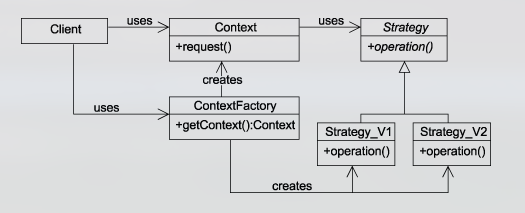
\includegraphics[scale=0.5]{strategy-pattern.png}
\caption{The variation of the Strategy Pattern used in this project, with creational logic is encapsulated in a factory class. Generic classnames shown here (e.g. Strategy) are specified in the report body. Source: Figure B.54 in Bain, 2008\cite{bain_emergent_2008}}
\label{fig:strategy-pattern}
\end{figure}

The design is encapsulated because the various versions of the behavior, how many variations there are, which variation will be used under a given circumstance, and the design of each varying implementation are all hidden from the client. We may also encapsulate the fact that the behavior is varying at all, depending on implementation.

\section{Conclusions}

Speech data analysis is confronted with novel complications, relative to text data analysis, in the adaptation of information-rich corpora varying across language, dialect, and formatting conventions for general linguistic analysis. Many of these complications produce dynamic problems for speech researchers, often resolved through informal scripting and manual data entry, that are well-suited to designed software tools. \\

This report documents work undertaken over a semester in the MCQLL Lab to experiment with and extend the usage of existing software tools to the problems of generalized speech data corpora preparation and analysis; particularly to the preparation problems of corpora storage and speech-text alignment. The existing storage and speech-text alignment tools used are PolyglotDB and Montreal Forced Aligner respectively. The steps taken to use these tools for facilitation of a pipeline, from publicly-available corpora acquisition to concrete linguistic analysis, is described technically, demonstrated experimentally, and documented in this report. This report constitutes a technical description of work undertaken with these tools for reproduction, reuse, and as a basis for streamlining the investigation of more advanced linguistics problems that require similar speech data preparation and analysis techniques. \\

This report additionally describes the software design approaches taken throughout the experimental process to motivate the contribution of the set of tools written by the author and to document their workings for future users, experimenters and developers. These tools are made available in a public repository. Alongside PolyglotDB and Montreal Forced Aligner, they facilitate the generalization of the experimental procedure taken across corpora and languages beyond those covered in the report experiments. This generalization is accomplished by abstracting the differences between corpora (varied in format and language) to a set of configuration files adaptable to the requirements of large sets of known public corpora. Differences in corpora that cannot be abstracted to configuration, especially morphological differences in syllable representation across languages, are implemented using a pattern-based approach, streamlining the introduction of new client logic for new corpora to the adaptation of a testable and flexible template class. This approach aims to contribute a code-base that can dynamically adapt to and reliably implement future client requirements when new corpora necessitate novel business logic in configuration and linguistic structure. \\

The design approach described arose emergently from the set of challenging problems produced by the varied and rich nature of speech data corpora. These problems surround the automation of various steps in corpora preparation for storage, alignment, and analysis: transcript encoding, audio signal processing, and pronunciation dictionary convention generalization. These problems and their relation to the problems of speech data alignment, storage, and analysis are described in this report, alongside the software contributed to resolve these problems. \\

Overall, this report describes an approach and some software solutions to aid in the resolution, by non-expert and expert researchers alike, of preparing publicly available speech data for alignment, storage, and analysis using publicly available tools. \\

\subsection{Acknowledgements}

My supervisor Morgan, my advisor Ann, my mentor Jasmine, my partner Ma\"ia, and cherished family, colleagues, comrades, teachers, and friends who have all supported me in innumerable ways along the way.

\newpage
\section{Appendix}
\subsection{Extra Figures}
\begin{figure}[h]
  \centering
  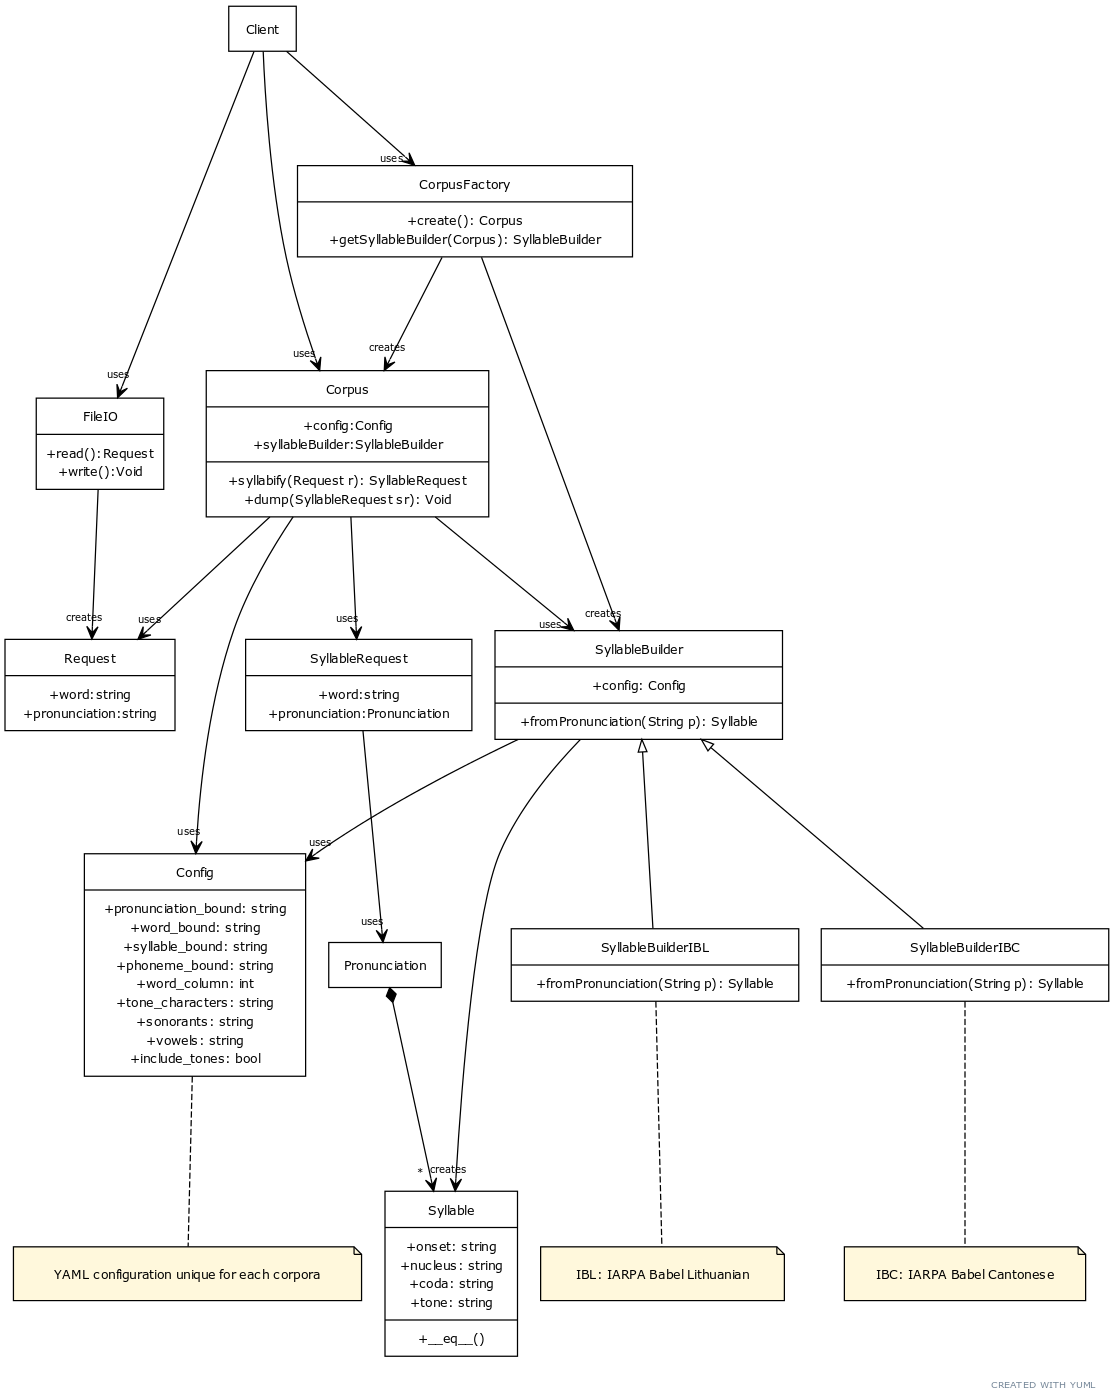
\includegraphics[scale=0.3]{UMLdiag.png}
  \caption{The complete UML diagram for the syllabification system produced during this project. The Strategy Pattern components can be seen in the Corpus/SyllableBuilder/Client relationships: the client can choose syllabification at runtime using configuration (for elements common to all languages) and dynamic algorithmic support (for elements unique to each language requiring higher-order logic) provided by the pattern.}
  \label{fig:UMLdiag}
\end{figure}

\newpage

\vskip 0.2in
\bibliography{sample}

\end{document}
